\section{Theorie}
\label{sec:Theorie}

\subsection{Röntgenstrahlung}
Unter die Röntgenstrahlung fällt die elektromagnetische Strahlung, dessen 
Spektrum im Energiebereich oberhalb des ultravioletten Lichts liegt.
Ebenso wie der Franck-Hertz Versuch handelt es sich um einen Elektronenstoßexperiment.
Röntgenstrahlung entsteht, indem beschleunigte Elektronen, welche aus einem 
Glühdraht freigesetzt wurden, auf eine Anode beschleunigt werden. Kommt diese 
dort an, so kommt es zur Wechselwirkung: Es entsteht das Bremsspektrum und 
das charakteristische Röntgenspektrum, diese werden im Folgenden erklärt.

\subsection{Das Bremsspektrum}
Das Bremsspektrum kommt zustande, wenn sich das Elektron dem Coulombfeld des 
Atomkerns nähert. Durch die gemeinsame negative Ladung wird das Elektron 
immer stärker abgebremst, je näher es dem Atom kommt. Dabei wird ein Röntgenquant 
emittiert, welches maximal die gesamte kinetische Energie des Elektrons übertragen
bekommt. Dementsprechend handelt es sich hier um ein kontinuierliches Spektrum,
wie in \autoref{fig:1} zu sehen.
\begin{figure}[H]
    \centering
        \centering
        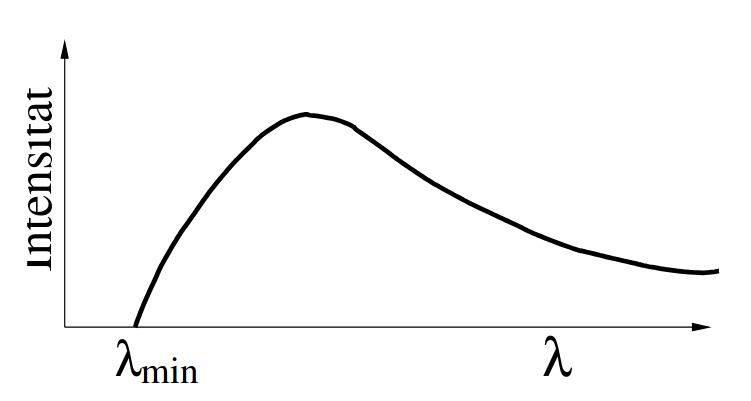
\includegraphics[width=0.7\textwidth]{bilder/brems.png}
        \caption{Bremssprektrum bei Röntgenstrahlung. \cite{anleitung10}}
    \hfill
    \label{fig:1}
\end{figure}
\noindent Die Energie wird aufgrund des Zusammenhangs von $E=h \nu$ maximal bei
der minimalen Wellenlänge, welche durch 
\begin{align}
    \lambda_{min} &= \frac{h c}{E} \\
                  &= \frac{h c}{e_0 U}
\end{align}
gegeben ist. Es fällt auf, dass das Spektrum gänzlich von der angelegten 
Beschleunigungsspannung abhängt.

\subsection{Das charakteristische Röntgenspektrum}
Im Gegensatz zum Bremsspektrum ist das charakteristische Spektrum nicht kontinuierlich.
Das liegt daran, dass es durch Ionisation des Atoms um diskrete Energieniveaus 
geht. Trifft ein Elektron mit genügend Energie auf das Atom, wird ein Elektron 
aus der inneren Schale gelöst. Im Folgezug rückt ein Elektron einer äußeren 
Schale nach um die Leerstelle zu eliminieren (Es entsteht eine diskrete 
Energiedifferenz von $E_m -E_n = h \nu$). Das geschieht bei Aussendung eines 
Röntgenquants bzw. Photons. Aufgrund der festen Energiedifferenz, setzt sich 
das Spektrum aus scharfen Linien zusammen (charakteristisch für Anodenmaterial),
welche durch die Buchstaben $K,L,M$ bezeichnet werden. Ein griechischer Buchstabe 
als Index gibt an, woher ein Elektron bei Rückfall kam. Beispielsweise steht 
$K_{\alpha}$ charakteristisch für einen Wechsel von der $L$-Schale auf die $K$-Schale 
und $K_{\beta}$ für den Wechsel von der $M$-Schale auf die $K$-Schale. Eine 
Veranschaulichung des Spektrums befindet sich in \autoref{fig:2}.
\begin{figure}[H]
    \centering
        \centering
        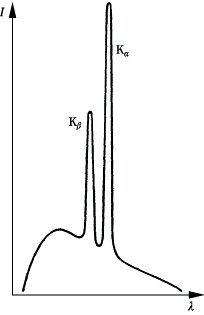
\includegraphics[width=0.3\textwidth]{bilder/char.jpg}
        \caption{Charakteristisches Röntgenspektrum. \cite{char}}
    \hfill
    \label{fig:2}
\end{figure}
\noindent In Mehrelektronenatomen erfährt ein äußeres Elektron nicht die volle Anziehungskraft 
des Kerns, da die inneren Elektronen einerseits abschirmen und andererseits 
die Abstoßung zwischen den Elektronen die Bindung zusätzlich schwächt. Dadurch 
wirkt auf das äußere Elektron eine reduzierte Kernladung, welche durch
\begin{equation}
    \sigma_{eff} = z - \sigma 
\end{equation}
definiert wird, $\sigma$ steht hierbei für die Abschirmkonstante.
Folglich verringert sich die Bindungsenergie, für diese gilt
\begin{equation}
    E_n = -R_{\infty} z_{eff}^2  \, \frac{1}{n^2}
\end{equation}
mit der Rydbergenergie $R_{\infty} = 13.6 \, \unit{\eV}$. Um ein Elektron aus 
dem Atom zu entfernen ergibt sich die Ionisationsenergie zu
\begin{equation}
    \label{eqn:a}
    E_{K,abs} = R_{\infty} (z - \sigma_1)^2.
\end{equation}
Für einen Übergang von der L-Schale auf die K-Schale gilt 
\begin{equation}
    \label{eqn:b}
    E_{K,\alpha} = R_{\infty} (z - \sigma_1)^2 \frac{1}{k} - R_{\infty} (z - \sigma_2)^2 \frac{1}{l}.
\end{equation}
Analog ist der Übergang von der M-Schale auf die K-Schale 
\begin{equation}
    \label{eqn:c}
    E_{K,\beta} = R_{\infty} (z - \sigma_1)^2 \frac{1}{k} - R_{\infty} (z - \sigma_3)^2 \frac{1}{m}
\end{equation}
mit $k = 1$, $l = 2$ und $m = 3$

\subsection{Absorption von Röntgenstrahlung}
Bei der Absorption von Röntgenstrahlung kommt es vor Allem zum Photoeffekt und 
dem Comptoneffekt: Das Photon wird vollständig absorbiert und ein Elektron 
rausgelöst. Zusätzlich treffen Photonen auf freie Elektronen, wobei Energie 
und Impuls an ein Elektron übertragen werden, wodurch sich die Wellenlänge 
vergrößert. Der Absorptionskoeffizient nimmt mit steigender Photonenenergie ab,
allerdings kann es zu Sprungstellen kommen, welche als Absorptionskanten $K,L$ 
bezeichnet werden, wie in \autoref{fig:3} zu sehen.
\begin{figure}[H]
    \centering
        \centering
        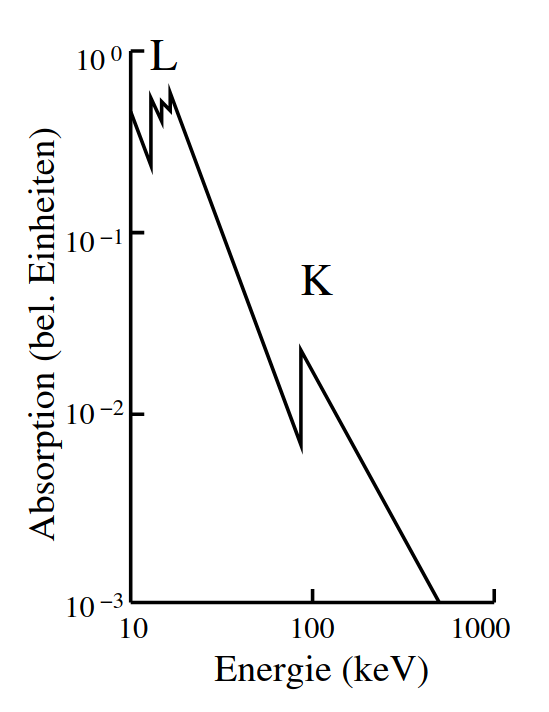
\includegraphics[width=0.3\textwidth]{bilder/ab.png}
        \caption{Darstellung der Absorptionskanten. \cite{anleitung10}}
    \hfill
    \label{fig:3}
\end{figure}
\noindent Während bei der $K$-Kante nur ein Peak vorliegt, gibt es drei bei der 
$L$-Kante. Jenes Phänomen ist mithilfe der Feinstruktur erklärbar. Um die
Bindungsenergie korrekt zu berechnen bedarf es der Sommerfeldschen Feinstrukturformel.
Aus dieser kann die Abschirmkonstante der K-Schale hergeleitet werden als 
\begin{equation}
    \label{sigma}
    \sigma_K = Z - \sqrt{\frac{E_K}{R_{\infty}} - \frac{\alpha^2 Z^4}{4}},
\end{equation}
wobei $Z$ die Ordnungszahl und $\alpha = \frac{1}{137}$ die Sommerfeldsche 
Feinstrukturkonstante ist.

\subsection{Bragg'sche Reflexion}
Als Bragg Winkel ist derjenige Winkekl definiert, bei dem Röntgenstrahlen 
konstruktiv interferieren. Das geschieht, indem das Röntgenlicht auf einen 
Kristall mit bekannter Gitterkonstante $d$ gelenkt und gebeugt werden. 
Mithilfe dieser Bragg-Reflexion kann die Wellenlänge und somit die Energie 
experimentell gemessen werden. Mit dem Winkel $\theta$ relativ zur Kristallebene 
und der Ordnungszahl $n$ der Reflexionsmaxima ist die Bragg'sche Reflektion 
definiert als folgender Term.
\begin{equation}
    2 d \sin(\theta) = n \lambda
\end{equation}

\subsection{Fehlerrechnung}
Die gemessenen Werte unterliegen Messunsicherheiten und werden demnach im
Folgenden nicht als fehlerfrei angesehen. Die Fehler entstehen bei der
Bildung der Mittelwerte durch den Fehler des Mittelwerts und bei der
Regressionsrechnung sowie der Fehlerforpflanzung durch Python.
Der Mittelwert ist definiert durch
\begin{equation}
    \overline{x} = \frac{1}{N} \sum\limits_{i=1}^N x_i.
\end{equation}
\noindent Der Fehler des Mittelwerts ist somit gegeben durch 
\begin{equation}
    \begin{aligned}
        \increment \overline{x} &= \sqrt{\overline{x^2\kern-0.1em} - \overline{x}^2} \\
                            &= \frac{\sqrt{\frac{1}{N-1} \sum\limits_{i=1}^N (x_i - \overline{x})^2}}{\sqrt{N}}.
    \end{aligned}
\end{equation}

Um Fehler einzubeziehen, wird die Gauß'sche Fehlerfortpflanzung verwendet:
\begin{equation}
    \label{eqn:9}
    \increment f = \sqrt{\left(\frac{\partial f}{\partial x}\right)^2 \cdot \left(\increment x\right)^2 + \left(\frac{\partial f}{\partial y}\right)^2 \cdot \left(\increment y\right)^2 + .... + \left(\frac{\partial f}{\partial z}\right)^2 \cdot \left(\increment z\right)^2}
\end{equation}